\lecture{1}{25. August 2025}{Introduction to Fluid Mechanics}

\section{Fundamental Concepts}

\subsection{Fluid as a Continuum}
Fluids are normally experienced as being continuous or ``smooth'' when percieved in the macroscopic world. If one looks at a fluid microscopically one would start to see that the fluid is not continuous at all but instead composed of distinct particles. We wish to determine the minimum volume, $\partial V'$ that a point $C$ must be such that we can talk about the fluid being continous at this point. In other words, under what circumstances can a fluid be treated as a continuum, for which, by definition, properties vary smoothly over all points. 

We define the mass $\partial m$ as the instantaneous number of molecules in $\partial V $ and the mass of each of these molecules. The average density inside volume $\partial V $ is hence given by $\rho = \frac{\partial m }{\partial V }$. It is important to note that this necessarily is an \textit{average value} as the number of molecules in $\partial V $ and hence the density fluctuates. Due to the law of large numbers one will experience that for very small volume the density will fluctuate greatly over time, however at a certain volume $\partial V' $, the density becomes stable and will not fluctuate greatly over time. For $\partial V = \qty{0,001}{mm^3}  $ (about the size of a grain of sand) there will already be an average of \num{2,5e13} molecules present. Hence a liquid can be treated as a continuous medium as long as we consider a ``point'' to be no smaller than about this size -- at least this is sufficiently precise for most engineering appplications.

This continuum hypothesis is an integral part of fluid mechanics. It is valid when treating the behaviour of fluids under normal conditions and only breaks down when the mean free path of the molecules becomes the same order of magnitude as the smallest characteristic dimension of the problem. 

As a consequence of the continuum assumption, each property of the fluid is assumed to have a definite value at each point in space. I.e. density, temperature, velocity, and so on are each continuous functions of both position and time. We now have a definition of the density at a point:
\[ 
\rho \equiv \lim_{\partial V \to \partial V'  } \frac{\partial m }{\partial V }
.\]
As point $C$ was chosen arbitrarily the density at any other point in the liquid can be determined in the same manner. If one measures this simultaneously for all points in the fluid, an expression for the density distribution as a function of the space coordinates $\rho = \rho(x,y,z)$ can be found.

The density at a specific point may also vary with time. Therefore the complete representation of density, the so-called \textit{field representation}, can be written as:
\begin{equation} \label{eq:dens}
\rho = \rho(x,y,z,t)
\end{equation}
As density is a scalar quantity the field given by \autoref{eq:dens} is a scalar field. 

The density can also be expressed as the specific gravity, i.e. the weith compared to the maximum density of water, $\rho_{\mathrm{H}_2 \mathrm{O}} = \qty{1000}{\frac{kg}{m^3}} \text{ at } \qty{4}{\celsius} $. Thus the specific gravity of a substance can be found as:
\[ 
\mathrm{SG} = \frac{\rho}{\rho_{\mathrm{H}_2 \mathrm{O}}}
.\]

Another useful property is the \textit{specific weight}, $\gamma$, of a substance. It is defined as the weight of a substance per unit volume, i.e.:
\[ 
\gamma = \frac{mg}{V} \implies \gamma = \rho g
.\]

\subsection{Velocity field}
A very important property defined by a field is the velocity field, given by:
\begin{equation} \label{eq:velo}
  \textbf{V} = \textbf{V}(x, y, z, t)
\end{equation}
As velocity is a vector quantity, the field given in \autoref{eq:velo} is a vector field.

The velocity vector, $\textbf{V}$, can also be written in terms of its scalar components. Denoting the components in the $x$-, $y$-, and $z$-directions by $u$, $v$, and $w$, respectively we get:
\[ 
\textbf{V} = u \hat{i} + v \hat{j} + w \hat{k}
.\]
Here, each component, $u$, $v$, and $w$, will generally be functions of $x$, $y$, $z$ and $t$.

We also need to be make sure to remember that $\textbf{V}(x, y, z, t)$ represents the velocity of a fluid particle passing through the point $(x,y,z)$ at time $t$. Therefore $\textbf{V}(x,y,z,t)$ should be thought of as the velocity field of the entire fluid and not of an individual particle.

If properties at every point in a flow field are constant with respect to time, the flow is termed \textit{steady}. This is defined mathematically as:
\[ 
\frac{\partial \eta}{\partial t} = 0
.\]
Where $\eta$ is any fluid property. Hence, for steady flow:
\[ 
\frac{\partial \rho}{\partial t} = 0 \text{ or } \rho = \rho(x,y,z)
\]
and
\[ 
\frac{\partial \textbf{V}}{\partial t} = 0 \text{ or } \textbf{V} = \textbf{V}(x,y,z)
.\]
As such any property may vary from point to point in the field but remain constant with time at every point for steady flow. 


\subsection{One-, Two-, and Three-Dimensional flows}
A flow is either one-, two-, or three-dimensional depending on the amount of spatial coordinates required to specify the velocity field. \autoref{eq:velo} shows that the velocity field in some cases is a function of three spatial coordinates and time -- in this case it is a three-dimensional flow.

Almost all flows are three-dimensional in nature -- however, analysis based on fewer dimensions is often sufficient. The complexity of analysis increases sharply as more dimensions are added, and oftentimes in engineering a one-dimensional analysis is sufficient. 

To not break the continuum assumption all fluids must have zero velocity at any solid surface, e.g. the inner side of a pipe. Due to this all flow in pipes is inherently three-dimensional. To simplify the analysis one often uses the notion of \textit{uniform flow} at a given cross-section. In a flow that is uniform at a given cross-section, the velocity is constant across any section normal to the flow as shown in \textbf{\autoref{fig:f2_3}}. Under this assumption, the flow simplifies to be simply a function of $x$ alone. The term \textit{uniform flow field} is used to describe a flow in which the velocity is constant throughout the entire field.

\begin{figure} [ht]
  \centering
  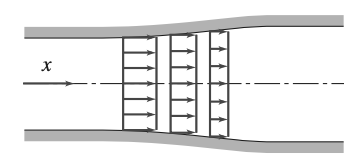
\includegraphics[width=0.5\linewidth]{./figures/f2_3.png}
  \caption{\textit{Uniform flow} at a given cross-section.}
  \label{fig:f2_3}
\end{figure}

\begin{definition}[Uniform flow at a cross section]
  An assumption that states that a fluid has the same velocity everywhere in a given cross section as shown on \textbf{\autoref{fig:f2_3}}. This actually breaks the continuum hypothesis but it makes a lot of calculations easier.
\end{definition}

\begin{definition}[Uniform flow field]
  A flow field where the velocity is constant everywhere throughout the flow field.
\end{definition}


\subsection{Timelines, Pathlines, Streaklines, and Streamlines}
Wind tunnels have traditionally often utilized to visualize flow fields. In modern times the advent of computer simulations has meant that these have become much more prevalent recently. A few different terms must be defined for proper understanding of these.

\begin{definition}[Timeline]
  A \textit{timeline} is produced by marking adjacent fluid particles in a flow field at a given instant. Subsequent observation of the timeline can give insights into the flow field.
\end{definition}

\begin{definition}[Pathline]
  A \textit{pathline} is the trajectory traced out by a moving fluid particle. These can be visualized by marking a fluid particle at a given instant, e.g. with dye or smoke, and then tracing the path of this particle as it moves through the field.
\end{definition}

\begin{definition}[Streakline]
  A \textit{streakline} is the line traced out by marking the fluid particles at a fixed point in space, e.g. with smoke or dye. This is therefore a way to see how fluid particles that passed through a specific point behave afterwards.
\end{definition}

\begin{definition}[Streamlines]
  A \textit{streamline} are lines drawn in a flow field such that at any given instant they are tangent to the velocity vector at every point in the flow. This means there can be no flow across a streamline. These are the most commonly used visualization technique
\end{definition}

We can use the velocity field to derive the shapes of streaklines, pathlines and streamlines. As the streamlines are parallel to the velocity vector, for a two dimensional flow field, we can write:
\begin{equation} \label{eq:stre}
  \frac{\mathrm{d}y}{\mathrm{d}x} \bigg|_{\text{streamline}} = \frac{v(x,y)}{u(x,y)}
\end{equation}
Note that these are obtained at a given instant in time. If the flow is unsteady, time $t$ is held constant in \textbf{\autoref{eq:stre}}. Solution of the equation gives $y = y(x)$, with an undetermined integration constant, the value of which depends on the particular streamline.

For pathlines, we let $x = x_p(t)$ and $y = y_p(t)$ where $x_p(t)$ and $y_p(t)$ are the instantaneous coordinates of a specific particle. In this case we get
\begin{equation} \label{eq:path}
  \frac{\mathrm{d}x}{\mathrm{d}t} \bigg|_{\text{particle}} = u(x,y,t) \qquad \frac{\mathrm{d}y}{\mathrm{d}t} \bigg|_{\text{particle}} = v(x,y,t)
\end{equation}
The simultaneous solution of these equations gives the path of a particle in parametric form, $x_p(t), y_p(t)$.

For streaklines, the first step is to compute the pathline of a particle with \autoref{eq:path} that was released from the streak source at $x_0$, $y_0$ at time $t_0$, in the form
\[ 
x_{\text{particle}} (t) = x(t, x_0, y_0, t_0) \qquad y_{\text{particle}}(t) = y(t, x_0, y_0, t_0)
.\]
Then now, instead of interpreting this as the position of a particle over time, we instead write the equations as:
\begin{equation}\label{eq:streak}
  x_{\text{streakline}} \left( t_0 \right) = x \left( t, x_0, y_0, t_0 \right) \qquad y_{\text{streakline}} \left( t_0 \right) = y \left( t, x_0, y_0, t_0 \right)
\end{equation}
\autoref{eq:streak} gives the line generated (by time $t$) from a streak source placed at $(x_0, y_0)$. In these equations $t_0$ is varied from $0$ to $t$ to show the \textit{instantaneous} positions of all particles released up to time $t$. 

\subsection{Stress Field}
To understand the behaviour of fluids one must first understand the nature of the forces that act upon fluid particles. A fluid particle can experience either:
\begin{itemize}
  \item \textit{Surface forces}, e.g. pressure or friction, that are generated due to contact with other particles or surfaces
  \item \textit{Body forces}, e.g. gravity and electromagnetic, that are experienced throughout the particle.
\end{itemize}

Surface forces on a fluid particle leads to \textit{stresses}. Stress is an important concept when describing how forces acting on the boundaries of a medium are transmitted throughout the medium. 

We consider the surface of a particle in contact with other fluid particles and the contact force being generated between these. Let $\delta \textbf{A}$ be a portion of the surface at some point $C$. The orientation of $\delta \textbf{A}$ is given by the unit vector $\hat{n}$, which is perpendicular to the surface as seen in \textbf{\autoref{fig:f2_6}}.

The force, $\delta \textbf{F}$, acting on the surface portion $\delta \textbf{A}$ may be split into two components -- a \textit{normal stress} $\sigma_n$ normal to the surface and a \textit{shear stress} $\tau_n$ tangential to the surface, defined as:
\begin{align*}
  \sigma_n &= \lim_{\sigma A_n \to 0} \frac{\delta F_n}{\delta A_n} \\
  \tau_n &= \lim_{\delta A_n \to 0} \frac{\delta F_t}{\delta A_n}
.\end{align*}

The subscript $n$ on the stress is a reminder that the stresses are associated with the surface portion $\delta \textbf{A}$ through $C$, which has an outward normal in the $\hat{n}$ direction. 

\begin{figure} [ht]
  \centering
  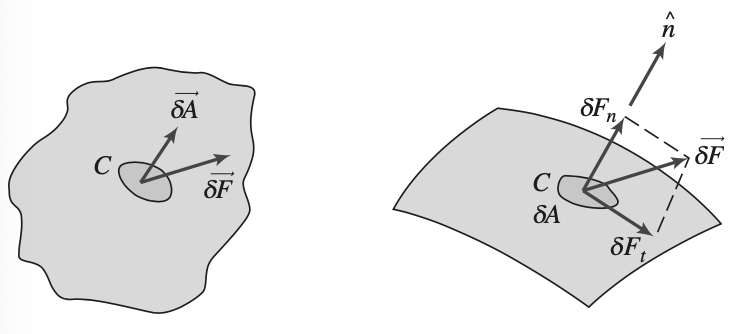
\includegraphics[width=0.5\linewidth]{./figures/f2_6.png}
  \caption{Stress in a continuum.}
  \label{fig:f2_6}
\end{figure}

We consider the stress on the element $\delta A_x$ whose normal is in the $+x$-direction. We can then split the force acting upon this point $\delta \textbf{F}$ into components along each coordinate direction. By dividing the magnitude of each force component by the area $\delta A_x$ and taking the limit as $\delta A_x$ approaches zero we define three stress components as:
\begin{align*}
  \sigma_{ x x} &= \lim_{\delta A_x \to 0} \frac{\delta F_x}{\delta A_x} \\
  \tau_{xy} &= \lim_{\delta A_x \to 0} \frac{\delta F_y}{\delta A_x} \\
  \tau_{xz} &= \lim_{\delta A_x \to 0} \frac{\delta F_z}{\delta A_x}
.\end{align*}
This is also shown graphically in \textbf{\autoref{fig:f2_7}}.

\begin{figure} [ht]
  \centering
  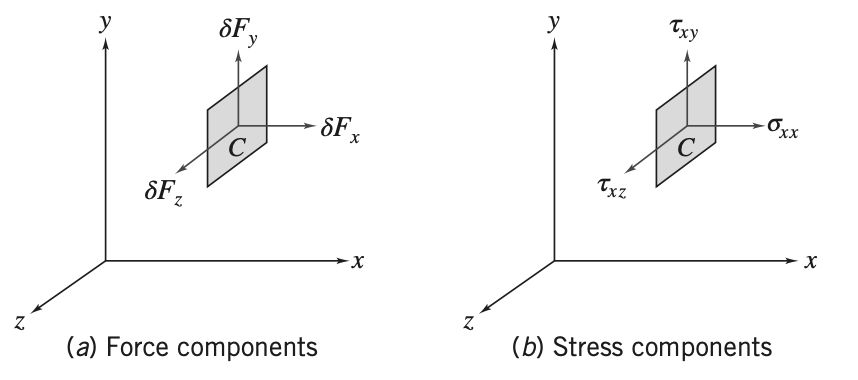
\includegraphics[width=0.5\linewidth]{./figures/f2_7.png}
  \caption{Force and stresses at surface element $\delta A_x$}
  \label{fig:f2_7}
\end{figure}

Here the first subscript ($x$) indicates the \textit{plane} on which the stress acts, in this case a surface perpendicular to the $x$-axis. The second direction indicates the \textit{direction} in which the stress acts. I.e. consideration of the element $\delta A_y$ would lead to the stresses $\sigma_{yy}$, $\tau_{yx}$ and $\tau_{yz}$ and similarly for $\delta A_{z}$. 

As the coordinate system was chosen arbitrarily it is easily realized that one can define an infinite amount of stresses through a point $C$ depending on how the axes are placed. Luckily, the state of stress at any point is completely described by the stresses acting in any three mutually perpendicular planes through the point. Therefore the stress at a point is specified by the nine components:
\[ 
\begin{bmatrix}
\sigma_{x x} & \tau_{xy} & \tau_{xz}\\
\tau_{yx} & \sigma_{yy} & \tau_{yz}\\
\tau_{z x} & \tau_{zy} & \sigma_{zz}\\
\end{bmatrix}
.\]
Planes are normally named for the direction in which their normal vector is pointing. Also we normally define a stress component to be positive when the stress component and the plane on which it acts are either both positive or negative.

\subsection{Viscosity}
For a solid stresses develop when the material is elastically deformed or strained; for a fluid, shear stresses instead arise due to viscosity. For a fluid at rest there will be no shear stresses.

We consider the behaviour of a fluid element between two infinite planes sketched on \textbf{\autoref{fig:f2_9}}. The rectangular fluid element is initially at rest at time $t$. We now suppose a constant rightward force $\delta F_x$ is applied to the upper plate such that it is dragged across the fluid at constant velocity $\delta u$. The shearing action of the plates produces a shear stress $\tau_{yx}$, which acts on the fluid element, and is given by:
\[ 
\tau_{yx} = \lim_{\delta A_y \to 0} \frac{\delta F_x}{\delta A_y} = \frac{\mathrm{d} F_x}{\mathrm{d}A_y} 
\]
where $\delta A_y$ is the contact area between the fluid element between the plade and $\delta F_x$ is the force exerted by the plate on the element.

\begin{figure} [ht]
  \centering
  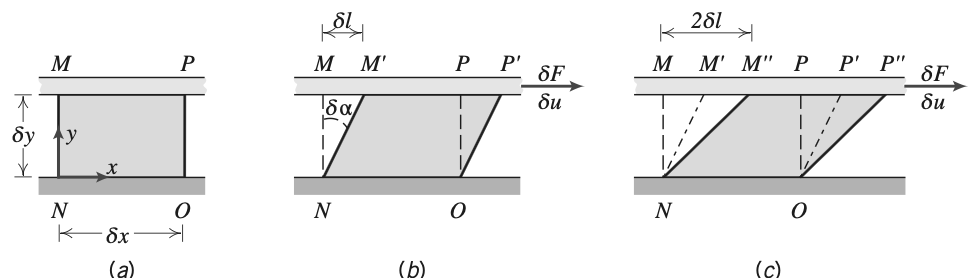
\includegraphics[width=0.5\linewidth]{./figures/f2_9.png}
  \caption{(a) Fluid element at time $t$, (b) deformation of fluid element at time $t + \delta t$, (c) deformation of fluid element at time $t + 2\delta t$}.
  \label{fig:f2_9}
\end{figure}

Focusing on the time interval $\delta t$ (\textbf{\autoref{fig:f2_9}b}) the deformation of the fluid is given by:
\[ 
\text{deformation rate} = \lim_{\delta t \to 0} \frac{\delta \alpha}{\delta t} = \frac{\mathrm{d} \alpha}{\mathrm{d}t} 
.\]

We will now seek to express $\frac{\mathrm{d}\alpha}{\mathrm{d}t} $ in terms of measurable quantities. The distance, $\delta l$, between the points $M$ and $M'$ is given by:

\[ 
\delta l = \delta u \delta t
.\]
For small angles this simplifies to:
\[ 
\delta l = \delta y \delta \alpha
.\]

Equating these two expressions gives:
\[ 
\frac{\delta \alpha}{\delta t} = \frac{\delta u}{\delta y}
.\]
By taking the limits of both sides of this, we get:
\[ 
\frac{\mathrm{d}\alpha}{\mathrm{d}t} = \frac{\mathrm{d}u}{\mathrm{d}y} 
.\]
Thus, the fluid element will, when subjected to a shear stress $\tau_{yx}$, experience a rate of deformation given by $\frac{\mathrm{d}u}{\mathrm{d}y} $. We have thus established that any fluid will flow and have a shear rate when subjected to a shear stress. Fluids in which the shear stress is proportional to the deformation rate are termed \textit{Newtonian} and fluids for which this is not the case are termed \textit{non-Newtonian}.

\subsection{Newtonian Fluid}
Most common fluids are Newtonian under normal conditions. If the fluid on \textbf{\autoref{fig:f2_9}} is Newtonian, then:
\[ 
\tau_{yx} \propto \frac{\mathrm{d}u}{\mathrm{d}y} 
.\]
The constant of proportionality between these two quantities is the \textit{absolute viscosity} also called the dynamic viscosity, $\mu$. Thus in terms of the coordinates on \textbf{\autoref{fig:f2_9}} Newton's law of viscosity for one-dimensional flow is:
\begin{equation} \label{eq:newvisone}
  \tau_{yx} = \mu \frac{\mathrm{d}u}{\mathrm{d}y} 
\end{equation}
By dimensional analysis on \textbf{\autoref{eq:newvisone}} it can be seen that the units of viscosity are \unit{kg.\per.m.s} or \unit{Pa.s}.

In fluid mechanics the ratio of absolute viscosity $\mu$ to density $\rho$ often arises. This ratio is called the \textit{kinematic viscosity} and is represented by $\nu$. The units for this is $\qty{1}{stoke} \equiv \qty{1}{cm^2.\per.s}$.

\subsection{Non-Newtonian Fluids}
Many empirical equations have been proposed to model the observed relations between $\tau_{yx}$ and $\frac{\mathrm{d}u}{\mathrm{d}y} $ for time-independent non-Newtonian fluids. For many engineering applications the power law model is sufficient, for which one-dimensional flow becomes:
\[ 
\tau_{yx} = k \left( \frac{\mathrm{d}u}{\mathrm{d}y}  \right)^{n}
.\]
Here $n$ is called the \textit{flow behaviour index} and $k$ is called the \textit{consistency index}. Newton's law of viscosity is a special case of this with $n = 1$ and $k = \mu$. To ensure that $\tau_{yx}$ has the same sign as $\frac{\mathrm{d}u}{\mathrm{d}y} $ the equation is rewritten as:
\begin{equation} \label{eq:nonnewvisone}
  \tau_{yx} = k \left| \frac{\mathrm{d}u}{\mathrm{d}y}  \right|^{n-1} \frac{\mathrm{d}u}{\mathrm{d}y} = \eta \frac{\mathrm{d}u}{\mathrm{d}y} 
\end{equation}
Here the term $\eta = k \left| \frac{\mathrm{d}u}{\mathrm{d}y}  \right|^{n-1}$ is referred to as the \textit{apparent viscosity}. When using \textbf{\autoref{eq:nonnewvisone}} we end up with a viscosity $\eta$ that is used in a formula in the same form as \textbf{\autoref{eq:newvisone}}. The big difference between these two is that while $\mu$ is constant (at a constant temperature), $\eta$ depends on the shear rate.

Fluids for which the apparent viscosity decreases with increasing deformation rate ($n<1$) are called \textit{pseudoplastic} or shear thinning fluids. Most non-Newtonian fluids are of this type. If the apparent viscosity increases with deformation rate ($n>1$) the fluid is termed \textit{dilatant} or shear thickening.

A ``fluid'' that behaves as a solid until a minimum yield stress $\tau_y$ is exceeded and subsequently exhibits a linear relation between stress rate and deformation is termed an ideal or \textit{Bingham plastic}. The shear stress model for a Bingham plastic is:
\[ 
\tau_{yx} = \tau_y + \mu_p \frac{\mathrm{d}u}{\mathrm{d}y} 
.\]

The apparent viscosity may also be time-dependent. \textit{Thixotropic} fluids show a decrease in $\eta$ with time at a constant stress and \textit{Rheopectic} fluids show an increase in $\eta$ with time. Some fluids partially return to their original shape when the stress is removed -- these are called \textit{viscoelastic}.

\subsection{Surface Tension}
Droplets can either ``flatten out'' or remain as little drops when dropped on a surface. We define a liquid as \textit{wetting} a surface when the contact angle is $<\ang{90}$. This is shown on \textbf{\autoref{fig:f2_11}}.

\begin{figure} [ht]
  \centering
  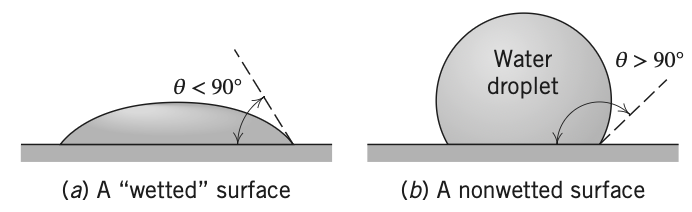
\includegraphics[width=0.5\linewidth]{./figures/f2_11.png}
  \caption{Surface tension effects on water droplets.}
  \label{fig:f2_11}
\end{figure}

Surface tension arises at the interface between the liquid and a solid -- this interface acts like a stretched elastic membrane in turn creating surface tension. This membrane is completely described by two features: the contact angle $\theta$ and the magnitude of the surface tension $\sigma \left[ \unit{N/m} \right]$. Both of these depend on both the type of liquid and the characteristics of the surface with which it shares an interface. 

\subsection{Description and Classification of Fluid Motions}
The two most difficult aspects of a fluid mechanics analysis to deal with are: (1) the fluid
s viscous nature and (2) its compressibility. When fluid mechanics first was developed it was occupied with a frictionless and incompressible fluid. Whilst extremely elegant this leads to the infamous result called d'Alembert's paradox, which states that all bodies experience zero drag as they move through a liquid -- which of course is not consistent with observations. 

\subsubsection{Viscous and Inviscid Flows}
Any object moving through a fluid will experience gravity and an aerodynamic drag force. This drag force is in part due to viscous friction and in part due to pressure differences being produced as the liquid moves out of the way of the object. We can estimate whether or not viscous forces are negligible compared to pressure forces by computing the Reynolds number:
\[ 
\mathrm{Re} = \rho \frac{VL}{\mu}
.\]
where $\rho$ and $\mu$ are the density and viscosity of the fluid, respectively, and $V$ and $L$ are the ``characteristic'' velocity and size scale of the flow, respectively. If the Reynolds number is ``large'' viscous effects will be small; however, if the Reynolds number is neither large nor small, both are important. 

The idealized notion of frictionless flow is called \textit{inviscid flow}. It predicts streamlines as shown in \textbf{\autoref{fig:f2_14}a}. These streamlines are symmetric front to back. As flow between two streamlines is constant the velocity in the vicinity of points $A$ and $C$ must be relatively low compared to the velocity at point $B$. Hence, points $A$ and $C$ have large pressures whereas $B$ will be a point of low pressure. In fact, the pressure distribution around the sphere is symmetric and there is therefore no net drag force due to pressure. As we are assuming inviscid flow there will be no drag force due to friction either -- this is the d'Alembert paradox of 1752.

\begin{figure} [ht]
  \centering
  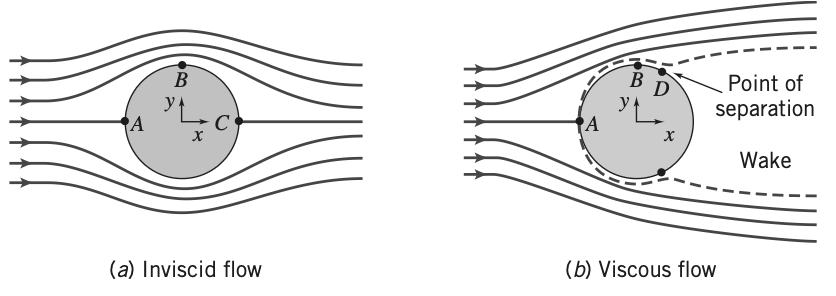
\includegraphics[width=0.5\linewidth]{./figures/f2_14.png}
  \caption{Incompressible flow over a sphere}
  \label{fig:f2_14}
\end{figure}

The answer to this was obtained by Prandtl in 1904. The no-slip condition requires that the velocity everywhere at the surface of the ball must be zero, but inviscid theory states that it is high at point $B$. Prandtl suggested that even though friction is negligible for high-Heynolds number flows, there will always be a thin boundary layer, in which friction is significant and over which the velocity will increase rapidly from zero at the surface to the value predicted by inviscid theory at the edge of the boundary layer. 

This thin boundary layer explains why drag arises. The boundary layer however also has another important consequence. It often leads to bodies moving through a fluid having a \textit{wake} as shown on \textbf{\autoref{fig:f2_14}b}. Here point $D$ is termed a \textit{separation point}, where fluid particles are pushed of the object thus creating the wake. It turns out that this wake always will have low pressure compared to the front of the sphere, hence the sphere now experiences quite a large \textit{pressure} or \textit{form drag}.

We can now also begin to see how \textit{streamlining} works. The main drag force in most aerodynamics is due to the low pressure wake. If we can reduce or even eliminate this wake the drag will be greatly reduced. Imagine that the sphere was instead teardrop shaped -- the pressure gradient will not be changing as quickly along the back half of the object and thus the wake will be smaller leading to less drag. This illustrates the \textit{very} significant different between inviscid flow ($\mu = 0$) and flows where the viscosity can be assumed negligible but not zero ($\mu\to 0$).

\subsubsection{Laminar and Turbulent flows}
A faucet turned on at a very low flow rate will lead to water running out smoothly -- if you increase the flow rate the water will exit in a much more chaotic manner. In fluid dynamics these are termed either \textit{laminar flow} or \textit{turbulent flow}. Oftentimes turbulence is unwanted but unavoidable.

The velocity of laminar flow is simply $u$. The velocity of turbulent flow is given by the mean velocity $\overline{u}$ plus the three components of randomly fluctuating velocity $u'$, $v'$, and $w'$. Many turbulent flows may be steady in the mean, but the presence of these random velocity fluctuations makes analysis of turbulent flows extremely difficult. In one-dimensional laminar flow, the shear stress is related to the velocity gradient by the simple relation:
\[ 
\tau_{yx} = \mu \frac{\mathrm{d}u}{\mathrm{d}y} 
.\]
For a turbulent flow, no such simple relation is valid. In turbulent flow momentum can be transported across streamlines and therefore there us no universal relationship between the stress field and the mean-velocity field. This means we often have to rely on semi-empirical theories for analyzing turbulent flow.

\subsubsection{Compressible and Incompressible Flows}
A flow in which the variation in density is negligible is termed \textit{incompressible} and those in which density variations are not negligible are called \textit{compressible}. Gasses are normally treated as compressible, whereas liquids are normally treated as incompressible. At high temperatures, however, compressibility effects can start to become important. Pressure and density changes in liquids are related by the \textit{bulk compressibility modulus} or the modulus of elasticity,
\[ 
E_v \equiv \frac{\mathrm{d}p}{\frac{\mathrm{d\rho}}{\rho}}
.\]
If the bulk modulus is independent of temperature, then density is only a function of pressure (the fluid is said to be \textit{barotropic}).

Gas flows with negligible heat transfer can be considered incompressible so long as the flow speeds are small relative to the speed of sound. The ratio of flow speed, $V$, to the local speed of sound, $c$, in the gas is defined as the Mach number:
\[ 
M \equiv \frac{V}{c}
.\]

For $M < \num{0,3} $ the maximum variation in density is less than 5\%. Thus gas flows with $M<\num{0,3} $ can be treated as being incompressible.


\subsubsection{Internal and External Flows}
Flows completely bounded by solid surfaces are called either \textit{internal}, \textit{pipe}, or \textit{duct flows}. Flows over bodies immersed in an unbounded fluid are termed \textit{external flows}.

An example of an internal flow is that of water in a pipe. The Reynolds number for pipe flows is defined as $\mathrm{Re} = \rho \overline{V} D / \mu$, where $\overline{V}$ is the average flow velocity and $D$ is the pipe diameter. Based on this one can predict if the flow will be laminar or turbulent. For $\mathrm{Re} < \num{2300} $ the flow will generally by laminar and turbulent for larger values. Flow in a pipe of constant diameter will always be entirely laminar or entirely turbulent, depending on the value of the velocity $\overline{V}$.
